\documentclass[tikz,border=2mm]{standalone}
\usepackage{tikz}
\usetikzlibrary{decorations.pathreplacing}


\begin{document}

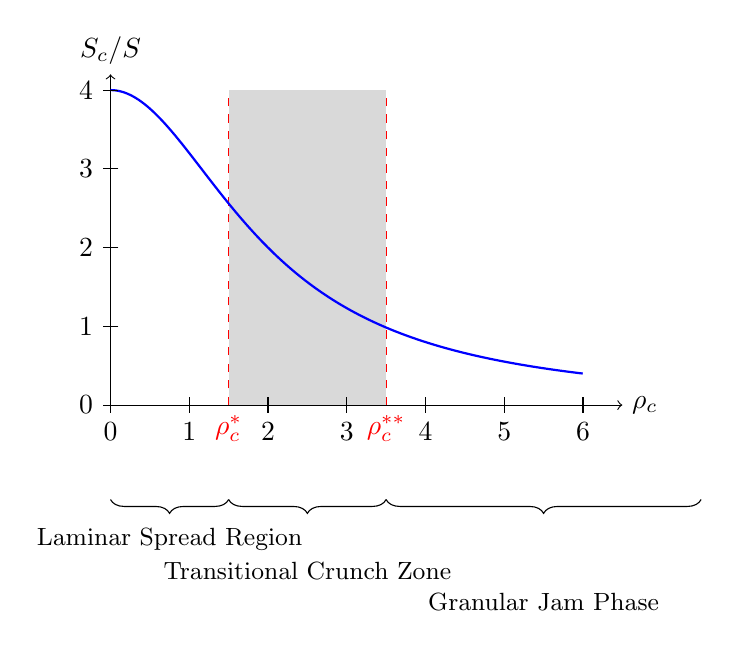
\begin{tikzpicture}[scale=1.0]
    % Axes
    \draw[->] (0,0) -- (6.5,0) node[right] {$\rho_c$};
    \draw[->] (0,0) -- (0,4.2) node[above] {$S_c/S$};

    % Dashed line for critical crunch density (left edge)
    \draw[dashed,red] (1.5,0) -- (1.5,4);
    \node[red] at (1.5, -0.3) {$\rho_c^*$};

    % Dashed line for critical crunch density (right edge)
    \draw[dashed,red] (3.5,0) -- (3.5,4);
    \node[red] at (3.5, -0.3) {$\rho_c^{**}$};

    % Shading for Transitional Crunch Zone
    \fill[gray!30] (1.5,0) rectangle (3.5,4);

    % Curve: S_c/S vs rho_c
    \draw[thick,blue,domain=0:6,smooth,samples=200] 
        plot (\x, {4/(1+((\x)/2)^2)});

    % X-axis ticks
    \foreach \x in {0,1,2,3,4,5,6}
        \draw (\x,0.1) -- (\x,-0.1) node[below] {\x};
    \foreach \y in {0,1,2,3,4}
        \draw (0.1,\y) -- (-0.1,\y) node[left] {\y};

    % Lower brackets with staggered labels
    \draw[decorate,decoration={brace,mirror,amplitude=5pt}] (0, -1.2) -- (1.5, -1.2) 
        node[midway,yshift=-0.5cm]{\small Laminar Spread Region};
    \draw[decorate,decoration={brace,mirror,amplitude=5pt}] (1.5, -1.2) -- (3.5, -1.2) 
        node[midway,yshift=-0.9cm]{\small Transitional Crunch Zone};
    \draw[decorate,decoration={brace,mirror,amplitude=5pt}] (3.5, -1.2) -- (7.5, -1.2) 
        node[midway,yshift=-1.3cm]{\small Granular Jam Phase};
\end{tikzpicture}

\end{document}

%%% Local Variables:
%%% mode: LaTeX
%%% TeX-master: t
%%% End:
